目前为止,工作项已经通过工作组本地内存交换数据,并通过隐式或显式barrier函数进行同步(这取决于内核是如何编写的),与工作组中的其他工作项进行了通信。\par

第4章中,讨论了另一种工作项分组。子工作组是工作组中定义子工作集,在相同的硬件资源或调度上一起执行。因为实现决定如何将工作项分组到子工作组中,子工作组中的工作项可能比任意工作组中的工作项更有效地通信或同步。\par

本节描述子工作组中工作项之间通信的构建块。注意,子工作组目前仅为ND-Range内核实现,并且子工作组不能通过分层内核表示。\par

\hspace*{\fill} \par %插入空行
\textbf{同步操作与子工作组的栅栏}

就像ND-Range内核中工作组中的工作项,可以使用工作组barrier功能进行同步,子工作组中的工作项可以使用子工作组栅栏功能进行同步。工作组同步可以通过调用工作项group\_barrier或nd\_item类的barrier功能完成。子工作组中的工作项的同步,是通过调用group\_barrier函数或sub\_group类上的barrier函数(可使用nd\_item类查询),如图9-11。\par

\hspace*{\fill} \par %插入空行
图9-11 查询和使用sub\_group类
\begin{lstlisting}[caption={}]
h.parallel_for(nd_range{{size}, {16}}, [=](nd_item<1> item) {
	auto sg = item.get_sub_group();
	...
	sg.barrier();
	...
});
\end{lstlisting}

像工作组栅栏一样,子工作组的栅栏可以接受参数,来更精确地控制栅栏操作。无论子工作组栅栏功能是同步全局内存还是本地内存,只同步子工作组中的工作项,都可能比同步工作组中的所有工作项要划算。\par

\hspace*{\fill} \par %插入空行
\textbf{子工作组内的数据交换}

与工作组不同,子工作组没有用于交换数据的专用内存空间。子工作组中的工作项可以通过工作组的本地内存、全局内存或通过使用子工作组集合函数来交换数据。\par

如前所述,集合功能是描述由一组工作项执行的操作的功能,而不是单个工作项,并且因为栅栏同步功能是由一组工作项执行的操作,所以是集合功能。\par

其他集合功能表示公共通信模式。我们将在本章后面详细描述许多集合函数,现在简要描述广播集合函数,将使用子工作组来实现矩阵乘法。\par

广播集合函数从组中的一个工作项中获取值,并将其传递给组中的所有其他工作项,配置示例如图9-12所示。注意,广播函数的语义要标识组中哪个值要通信的local\_id对于组中的所有工作项必须相同,以确保广播函数的结果对于组中的所有工作项是相同的。\par

\hspace*{\fill} \par %插入空行
图9-12 广播功能
\begin{center}
	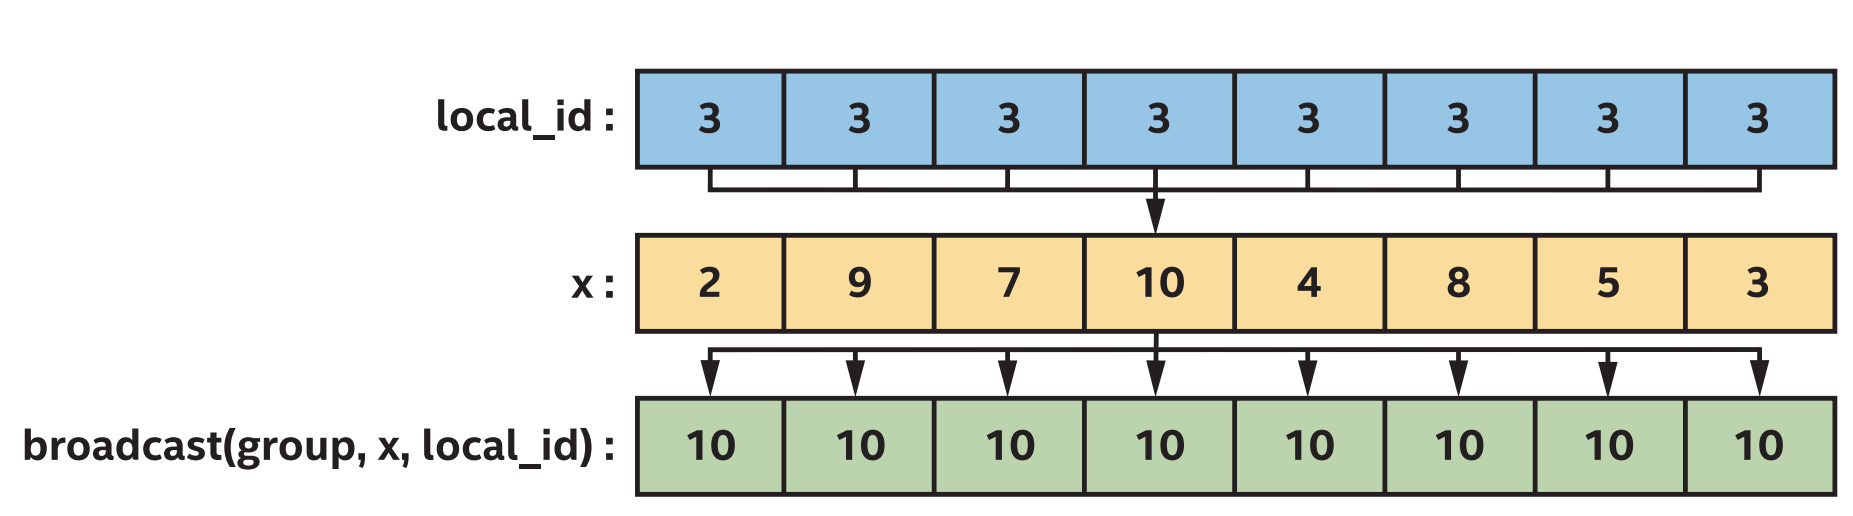
\includegraphics[width=1.\textwidth]{content/chapter-9/images/7}
\end{center}

如果查看本地内存矩阵乘法内核的最内层循环,如图9-13所示,可以看到对矩阵块的访问是一个广播操作,因为组中的每个工作项从矩阵块中读取相同的值。\par

\hspace*{\fill} \par %插入空行
图9-13 包含广播操作的矩阵乘法内核
\begin{lstlisting}[caption={}]
h.parallel_for<class MatrixMultiplication>(
	nd_range<2>{ {M, N}, {1, tileSize} }, [=](nd_item<2> item) {
	...
	
	// Perform computation using the local memory tile, and
	// matrix B in global memory.
	for( size_t k = 0; k < tileSize; k++ ) {
		// Because the value of k is the same for all work-items
		// in the group, these reads from tileA are broadcast
		// operations.
		sum += tileA[k] * matrixB[kk + k][n];
	}
	...
});
\end{lstlisting}

使用子组广播功能来实现不需要工作组本地内存或栅栏的矩阵乘法内核。许多设备上,子工作组广播比使用工作组本地内存和栅栏的广播更快。\par

\hspace*{\fill} \par %插入空行
\textbf{完整的子组ND-Range内核示例}

图9-14使用子工作组实现矩阵乘法的完整示例。注意,此内核不需要工作组本地内存或显式同步,而是使用子工作组广播集合函数在工作项之间通信矩阵块的内容。\par

\hspace*{\fill} \par %插入空行
图9-14 用NDrange parallel\_for和子组集合函数表示块矩阵乘法内核
\begin{lstlisting}[caption={}]
// Note: This example assumes that the sub-group size is 
// greater than or equal to the tile size!
static const int tileSize = 4;

h.parallel_for(
nd_range<2>{{M, N}, {1, tileSize}}, [=](nd_item<2> item) {
	auto sg = item.get_sub_group();
	
	// Indices in the global index space:
	int m = item.get_global_id()[0];
	int n = item.get_global_id()[1];
	
	// Index in the local index space:
	int i = item.get_local_id()[1];
	
	T sum = 0;
	for (int_fast64_t kk = 0; kk < K; kk += tileSize) {
		// Load the matrix tile from matrix A.
		T tileA = matrixA[m][kk + i];
		
		// Perform computation by broadcasting from the matrix
		// tile and loading from matrix B in global memory. The loop
		// variable k describes which work-item in the sub-group to
		// broadcast data from.
		for (int k = 0; k < tileSize; k++)
			sum += intel::broadcast(sg, tileA, k) * matrixB[kk + k][n];
	}

	// Write the final result to global memory.
	matrixC[m][n] = sum;
});
});
\end{lstlisting}



































